\documentclass{article}[18pt]
\usepackage{../../../../../format}
\lhead{MCS - LDS}


\begin{document}
\begin{center}
\underline{\huge Methods of Proof}
\end{center}
\section{Mathematical Proof}
A mathematical proof is a valid argument that establishes the truth of a mathematical argument\\
\\
A proof is generally constructed using:
\begin{itemize}
	\item The hypothesis of the theorem
	\item Axioms known to be true
	\item Previously proved theorems
	\item Rules of inference
\end{itemize}
Up until now, we have been considering formal proofs (in logics)\\
Now we focus on informal proofs, as applied by humans
\section{Theorems}
Theorems are usually stated using an informal version of first-order logic and often have one of the following structures:
\begin{itemize}
	\item "Every x is a y"
	\item "There is a x that is not y"
	\item "If something is x then it is a y"
\end{itemize}
Consequently, in order to prove many theorems we utilize our knowledge of first order logic\\
Different proof methods are available to us, often depending on the structure of the theorem to be proved
\section{Direct Proofs}
A direct proof is used to prove theorems of the form
\begin{center}
	\textit{If such and such then such and such}
\end{center}
More generally, theorems of the form
$$\forall x(P(x)\Rightarrow Q(x))$$
Essentially, a direct proof is a list of statements starting from P(x) and ending at Q(x), and where every statement in the list is
\begin{itemize}
	\item An axiom
	\item A previously proved theorem, or
	\item An inference of such using a rule of inference
\end{itemize}
Direct proofs, once stated, tend to be easy to check, but often some insight is required to devise the proof in the first place
\subsection{Example 1}
\subsubsection{Theorem}
If n is an odd integer then so is $n^2$
\subsubsection{Proof}
\begin{itemize}
	\item Suppose that n is an odd integer
	\item So, $n=2k+1$, for some integer k
	\item Thus, $n^{2}=(2 k+1)^{2}=(2 k+1)(2 k+1)=4 k^{2}+4 k+1$
	\item When we divide $n^2$ by 2 we get $2k^2+2k$ remainder 1
	\item Thus, $n^2$ is odd
\end{itemize}
\subsection{Example 2}
\subsubsection{Theorem}
If $m$ and $n$ are perfect squares then so is $mn$
\subsubsection{Proof}
\begin{itemize}
	\item Suppose that m and n are perfect squares
	\item So, $m=a^2$, for some integer a, and $n=b^2$, for some integer b
	\item Thus, $mn=a^2b^2=(ab)^2$
	\item So mn is a perfect square
\end{itemize}
\section{Proof by contraposition}
Proofs by contraposition are generally used to prove theorems of the form:
$$\forall x(P(x)\Rightarrow Q(x))$$
The key to a proof by contraposition is the following argument from first-order logic
\begin{itemize}
	\item M is a model of $\forall x(P(x)\Rightarrow Q(x))$
	\item Iff for every x, M is a model of $P(x)\Rightarrow Q(x)$
	\item Iff for every x, M is a model of $\lnot Q(x)\Rightarrow \lnot P(x)$
	\item Iff M is a model of $\forall x(\lnot Q(x)\Rightarrow \lnot P(x))$
\end{itemize}
Thus, if we wish to prove that $\forall x(P(x)\Rightarrow Q(x))$ is a theorem, then it suffices to prove that for any value of x, $\lnot Q(x)\Rightarrow \lnot P(x)$
\subsection{Example 1}
\subsubsection{Theorem}
If n is an integer and 3n+2 is odd then n is odd
\subsubsection{Proof}
\textit{Wanting to show that if n is even, then $3n+2$ is even (the opposite)}
\begin{itemize}
	\item Assume the negation of what we want to prove; that is, assume that n is even
	\item So, n=2k, for some integer k
	\item Thus, $3n+2=6k+2$ is even
	\item Hence, if n is even then $3n+2$ is even; that is, if $3n+2$ is odd then $n$ is odd
\end{itemize}
Let's try and prove the result above with a \textbf{direct proof}\\
Suppose that $3n+2$ is odd; so, 3n+2=2k+1, for some integer k. So, $3n=2k-1$ is odd\\
It's not so clear as to how to proceed now, as we appear to be back where we started except we have that 3n is odd as opposed to 3n+2
\subsection{Example 2}
\subsubsection{Theorem}
If m and n are integers and mn is even then m is even or n is even
\subsubsection{Proof}
\textit{Wanting to prove that if m and n are odd then mn is odd}\\
Assume that m is odd and n is odd.\\
So, $m=2k+1$, for some integer k, and $n=2p+1$, for some integer p\\
Thus,
$$m n=(2 k+1)(2 p+1)=4 k p+2 k+2 p+1=2(2 k p+k+p)+1$$
Which is odd
\subsection{Example 3}
\subsubsection{Theorem}
If n is an integer and $n^3+5$ is odd then n is even
\subsubsection{Proof}
\textit{Wanting to prove that is n is off then $n^3+5$ is even}\\
Assume that n is odd; so, $n=2k+1$, for some integer k\\
Thus,
$$
\begin{aligned} n^{3}+5 &=(2 k+1)^{3}+5 \\ &=(2 k+1)\left(4 k^{2}+4 k+1\right)+5 \\ &=8 k^{3}+12 k^{2}+6 k+6 \\ &=2\left(4 k^{3}+6 k^{2}+3 k+3\right) \end{aligned}
$$
Which is even
\section{Which is the easiest method to use?}
The previous examples show that using one proof method can be easier than using another; but how do we decide which proof method to use?\\
There is no canonical answer: a good approach is to try a direct proof and if you struggle, try proof by contraposition
\subsection{Theorem}
The sum of two rational numbers are rational
\subsection{Proof}
Try a direct proof. Let x and y be rational numbers; so, let $x=a/b$ and let $y=c/d$, where a,b,c and d are integers. Thus, $x+y=a / b+c / d=a d / b d+b c / b d=(a d+b c) / b d$, which is rational, and so the direct proof works\\
\\
If we tried a proof by contraposition then we would start by considering the irrational sum of two numbers $x+y$. This would not be of very much help
\section{Proof by contradiction}
Suppose that we wish to prove that something, p say, is true.\\
Suppose we also know:
\begin{itemize}
	\item Something else, q say, to be false
	\item $\lnot p\Rightarrow q$ to be true
\end{itemize}
The only way that $\lnot p\Rightarrow q$ can be true when q is false is for p to be true. The above state of affairs results in a proof by contradiction\\
\\
Look more closely at a proof by contradiction\\
It proves that p is true but it does it non-constructively; that is, it does it not by building a proof that p is true but by showing that if p were false then we would be able to prove that something known to be false is true
\subsection{Example 1}
\subsubsection{Theorem}
$\sqrt{2}$ is irrational
\subsubsection{Proof}
Suppose that $\sqrt{2}$ is rational; that is, suppose that $\sqrt{2}=a/b$ where a and b are integers and where no integer apart from 1 divides both a and b.\\
\\
So, $2=a^2/b^2$, with $a^2=2b^2$ and $a^2$ even.\\
\\
So we have that a is even; that is, $a=2p$ for some integer p.\\
\\
Hence, $4p^2=2b^2$ with $b^2=2p^2$; in particular, $b^2$ is even.\\
\\
So $b$ is even; so, $b=2q$, for some integer q.\\
\\
This, 2 divides a and 2 divides b, which yields a contradiction.\\
\\
Hence, our original assumption that $\sqrt{2}$ is rational cannot be correct; that is, $\sqrt{2}$ is irrational
\subsection{Example 2}
\subsubsection{Theorem}
There is no rational number r for which $r^3+r+1=0$
\subsubsection{Proof}
Suppose that $r=a/b$ is rational, where a and b are integers having no common factor different from 1. So,
$$a^3/b^3+a/b+1=0$$
with
$$a^3+ab^2+b^3=0$$
As 0 is even
$$a^3+ab^2+b^3$$
is even\\
If a and b are odd then $a^3+ab^2+b^3$ is odd - contradiction\\
If a is odd and b is even, $a^3+ab^2+b^3$ is odd - contradiction\\
If a is even and b is odd, $a^3+ab^2+b^3$ is odd - contradiction\\
So, a and b have a common factor 2 - contradiction
\section{Proof of equivalence}
Proof of equivalence have the form $p\Leftrightarrow q$ and are usually structured into two parts $p\Rightarrow q$ and $q\Rightarrow p$
\subsection{Example 1}
\subsubsection{Theorem}
For any integer n, n if odd iff $n^2$ is odd
\subsubsection{Proof}
\textbf{(Direct Proof)}: If n is odd then $n=2k+1$, for some integer k.\\
So, $n^2=(2k+1)^2=4k^2+4k+1=2(2k^2+2k)+1$ is odd\\
\\
\textbf{(Proof by contraposition)}: Conversely, now we wish to prove that if $n^2$ is odd then n is odd.\\
Suppose than n is even; that is, $n=2k$, for some integer k. Thus, $n^2=(2k)^2=2(2k^2)$ is even
\subsection{Example 2}
\subsubsection{Theorem}
If x is a real number then the following are equivalent
\begin{enumerate}[label=(\roman*)]
	\item $x$ is rational
	\item $x/2$ is rational
	\item $3x-1$ is rational
\end{enumerate}
\subsubsection{Proof}
\begin{itemize}
	\item Suppose that (i) holds
	\begin{itemize}
		\item So, $x=a/b$ is rational and $x/2=a/2b$ is rational
		\item So (ii) holds
	\end{itemize}
	\item Suppose that (ii) holds
	\begin{itemize}
		\item S, $x/2=a/b$ is rational and $x=2a/b$ is rational
		\item So (i) holds
	\end{itemize}
	\item Suppose that (i) holds
	\begin{itemize}
		\item So, $x=a/b$ is rational and $3x-1=3a/b=1=(3a-b)/b$ is rational
		\item So (iii) holds
	\end{itemize}
	\item Suppose that (iii) holds
	\begin{itemize}
		\item So, $3x-1=a/b$ is rational and $x=(a+b)/3b$ is rational
		\item So (i) holds
	\end{itemize}
\end{itemize}
Thus:
\begin{itemize}
	\item $(i)\Leftrightarrow (ii)$
	\item $(i)\Leftrightarrow (iii)$
\end{itemize}
Hence
\begin{itemize}
	\item $(ii)\Rightarrow (i)$
	\item $(i)\Rightarrow (iii)$
	\item $(iii)\Rightarrow (i)$
	\item $(i)\Rightarrow (ii)$
\end{itemize}
So, $(ii)\Leftrightarrow(iii)$


\section{Proof by cases}
Sometimes the proof of a theorem can be split up into the separate proofs of a small number of different cases
\subsection{Example}
\subsubsection{Theorem}
For integers a,b and c
\begin{center}
	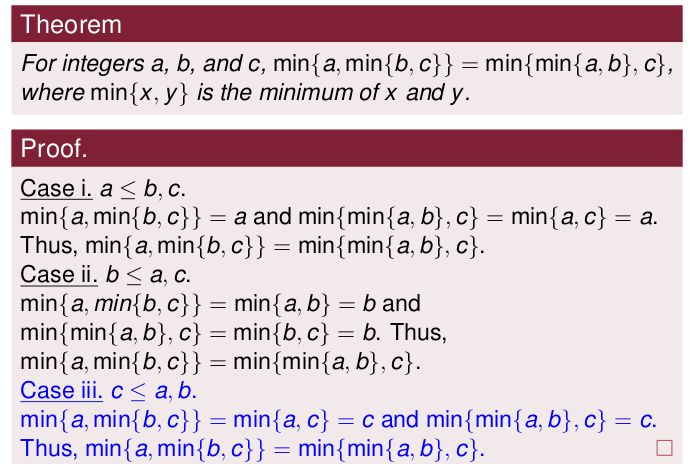
\includegraphics[scale=0.7]{cases}
\end{center}

\section{Exhaustive checks} 
Sometimes a proof by cases is nothing other than an exhaustive check
\subsection{Example}
\begin{center}
	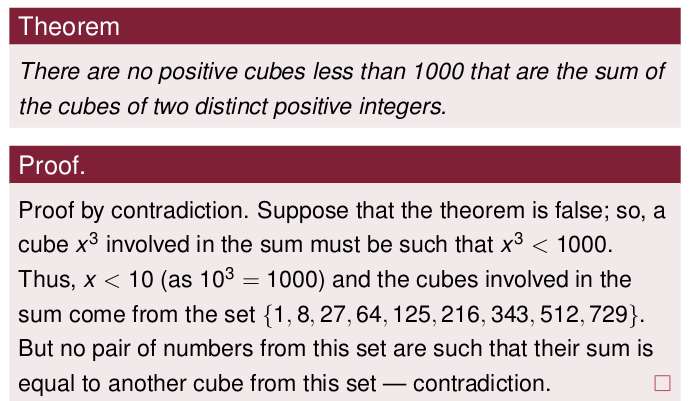
\includegraphics[scale=0.7]{exhaustive}
\end{center}

\section{Existence proofs}
Existence proofs tend to be proofs of theorems in the form $\exists x P(x)$\\
\\
In order to prove a theorem of the form $\exists x P(x)$ we can either construct an actual x such that $P(x)$ holds or we can show that such an x must exist without actually constructing it\\
The former are called constructive proofs, the latter non-constructive proofs\\
For example, in order to prove the theorem:\\
\textbf{Theorem}:\\
There is a positive integer that is the sum of all positive integers less than it\\
\\
We simply write $3=1+2$ to constructively prove this
\subsection{Non constructive existence proofs}
\begin{center}
	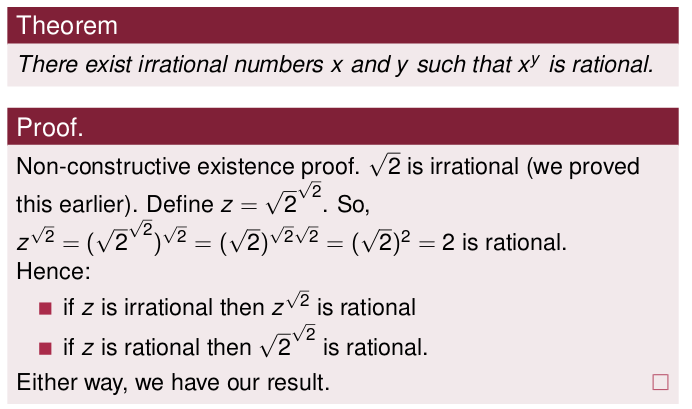
\includegraphics[scale=0.7]{existence}
\end{center}

\section{Proof by counterexample}
Consider a statement of the form $\forall x P(x)$\\
In order to prove it, we need to prove that for every x, P(x) holds\\
In order to disprove it, we need to find some x such that $\lnot P(x)$ holds (or, at least, show that such an x exists). That is, find (the existence of) a counterexample.\\
\\
For example, consider the statement
\begin{center}
	\textit{If a and b are rational numbers then $a^b$ is rational}
\end{center}
\textbf{Refutation.} Put $a=2$ and $b=1/2$. Then $a^b=\sqrt{2}$ is irrational.\\
Hence, the statement is not a theorem as we have found a counterexample




\end{document}